\documentclass[12pt,letterpaper]{article}

\usepackage[margin=0.75in,headheight=1.5em]{geometry}
\usepackage{graphicx}

\begin{document}
    \begin{center}
        {\Large\bf Robot Evactuation} \\
        \vspace{0.25em}
        {\large COMP 4001}\\
        \vspace{0.25em}
        Juhandr\'{e} Knoetze - 100882772 \\
    \end{center}

    \section{Implementation}
    \subsection{Pygame}
        Pygame is a graphics library developed for Python.
    
    \subsection{Classes}
        To implement the robot evacuation, multiple classes were used to represent the various parts of the scenario.
        
    \subsubsection{Robot}
        The Robot class is used to represent the robots in the evacuation. In the Robot class, it has attributes to hold the visual representation of the robot, as well as its coordinate location. There are also attributes to indicate if the robot has encounter the edge of the ring yet, or if it as evacuated.
        
        To create the visual component of the Robot, Pygame's Surface and Rect objects are used. A Robot has an instance of a Surface object which is the size of the Robot. The Surface object is what will be drawn on the screen to visually represent the Robot. A rectangle is drawn on the robot's surface of the chosen colour. The Rect instance returned from drawing on the Surface is kept by the Robot and is the object that will be manipulated when moving the Robot across the screen.
        
        Additional attributes held by the Robot class are properties such as
        
    \section{Algorithms}
    \subsection{Scenario 1}
        In the first scenario, both robots start in the center of the ring. To start the search for the exit, both robots go in the same direction until the perimeter. Once at the perimeter, the robots will go around the perimeter in opposite directions. If either robot finds the exit, the other robot is notified and the first robot will stop moving. When a robot is notified that the other has found the exit, it cuts the chord. The notified robot will leave the perimeter and head in a straight line towards the first robot.
        
%         \begin{center}
%             \frame{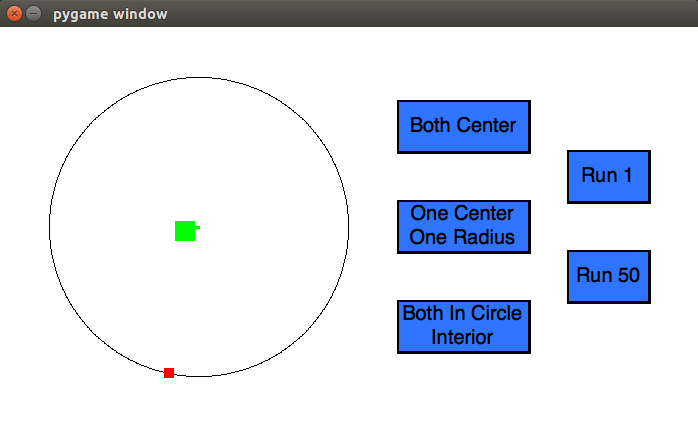
\includegraphics[scale=0.5]{images/scenario-1-1.png}}
%         \end{center}
%         
%         \begin{center}
%             \frame{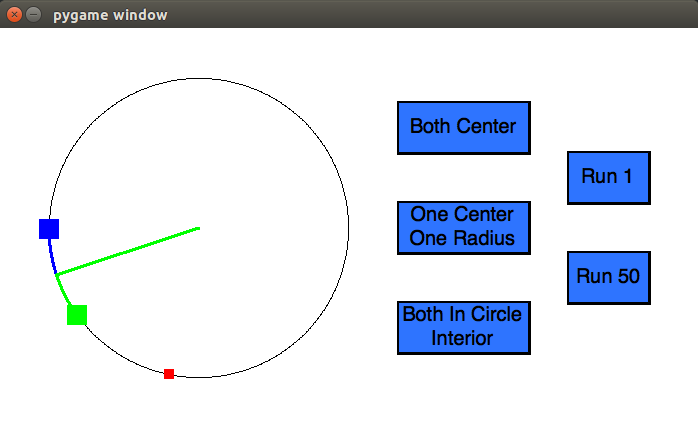
\includegraphics[scale=0.5]{images/scenario-1-2.png}}
%         \end{center}
%         
%         \begin{center}
%             \frame{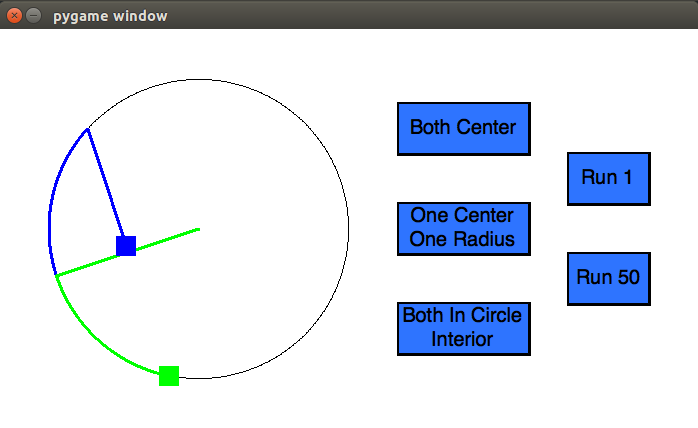
\includegraphics[scale=0.5]{images/scenario-1-3.png}}
%         \end{center}

        \begin{center}
            \frame{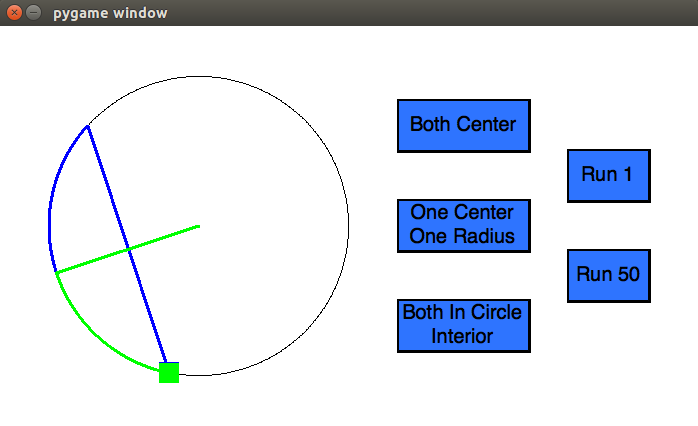
\includegraphics[scale=0.5]{images/scenario-1-4.png}}
        \end{center}

        \subsection{Scenario 2}
        In the second scenario, only one robot, robot $A$, will start in the center of the ring. The other, robot $B$, will be placed randomly in the ring. To evacuate the ring, both robots will go in the same direction towards the perimeter of the ring and start moving at the same time. The direction of travel will be such that robot $A$ is headed towards robot $B$. Since robot $A$ is in the center, it will always have to travel the radius of the ring regardless of where robot $B$ is placed. However, by traveling in that direction, robot $B$ will travel its shortest distance to the perimeter. Once the a robot reaches the perimeter, it will go in one direction and the other robot will always go in the opposite direction. This will ensure that the robots do not cover the same path along the radius, or else it would be equivalent to a single robot evacuation. Similarly to the first scenario, if a robot, say robot $A$, find the exit while searching the perimeter, it will stop moving and notify robot $B$. Robot $B$ will then cut the chord and head straight to the exit.
    
%         \begin{center}
%             \frame{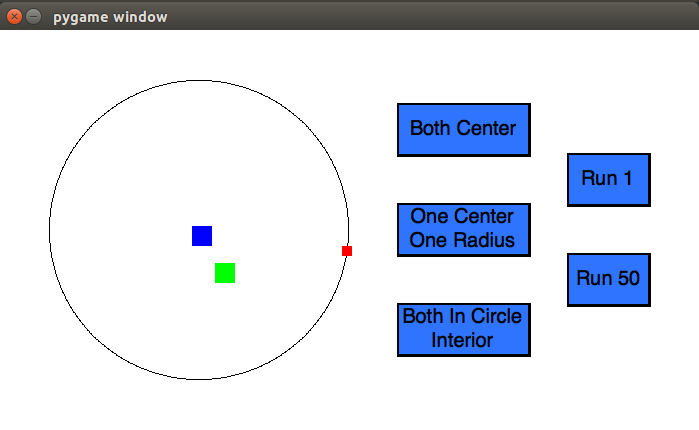
\includegraphics[scale=0.5]{images/scenario-2-1.png}}
%         \end{center}
%         
%         \begin{center}
%             \frame{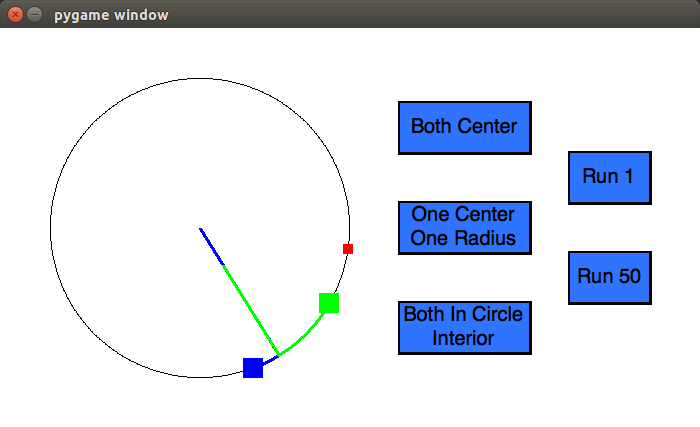
\includegraphics[scale=0.5]{images/scenario-2-2.png}}
%         \end{center}
%         
        \begin{center}
            \frame{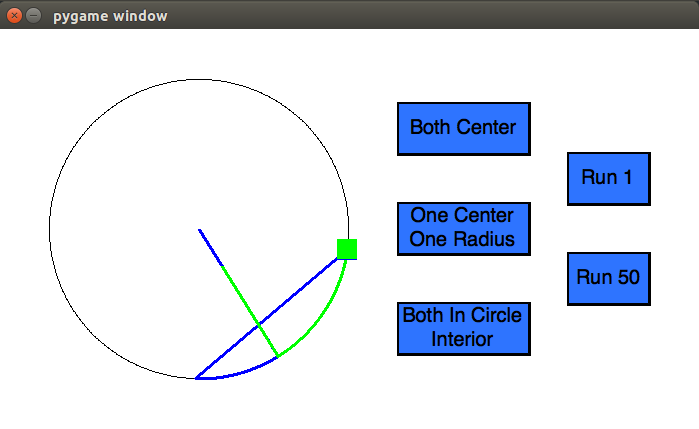
\includegraphics[scale=0.5]{images/scenario-2-3.png}}
        \end{center}
    
    \subsection{Scenario 3}
        In the third scenario, both robots are placed randomly in the circle. To get to the perimeter, the robots head a to a point on the perimeter that is equidistant from both robots. To find this point, the line between the two robots is calculated as well as the midpoint of that line. With the midpoint and line, the line for the perpendicular bisector can be calculated. The perpendicular bisector will intersect the perimeter of the ring at either 1 or 2 points. If it is one point, the robots will head to that one point. If it is two points, the robots will head to the closet point. Once at the perimeter, the rest of the evacuation is identical to the other two scenarios. Both robots head in opposite directions and if one robot finds the exit, the other will cut across the circle to go to the exit.
        
%         \begin{center}
%             \frame{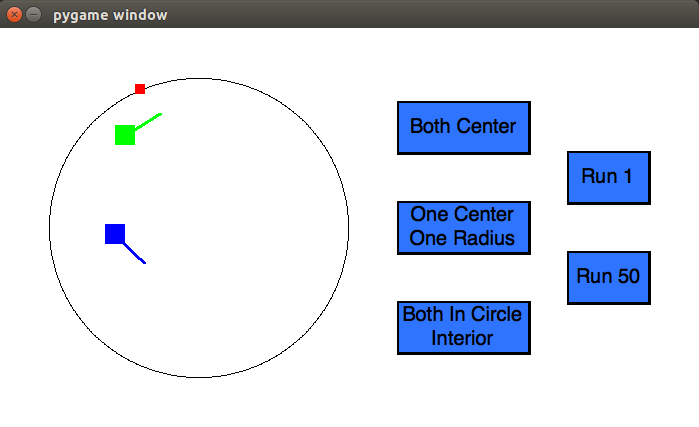
\includegraphics[scale=0.5]{images/scenario-3-1.png}}
%         \end{center}
%         
%         \begin{center}
%             \frame{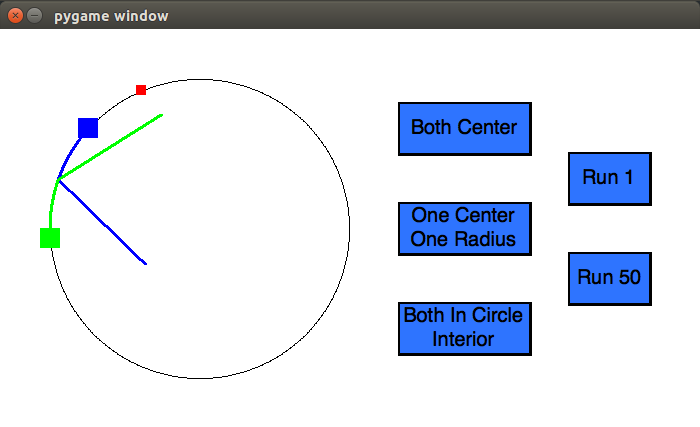
\includegraphics[scale=0.5]{images/scenario-3-2.png}}
%         \end{center}
%         
%         \begin{center}
%             \frame{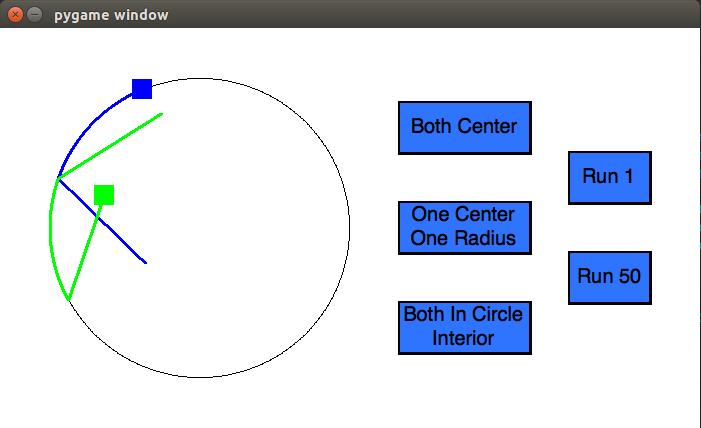
\includegraphics[scale=0.5]{images/scenario-3-3.png}}
%         \end{center}
%         
        \begin{center}
            \frame{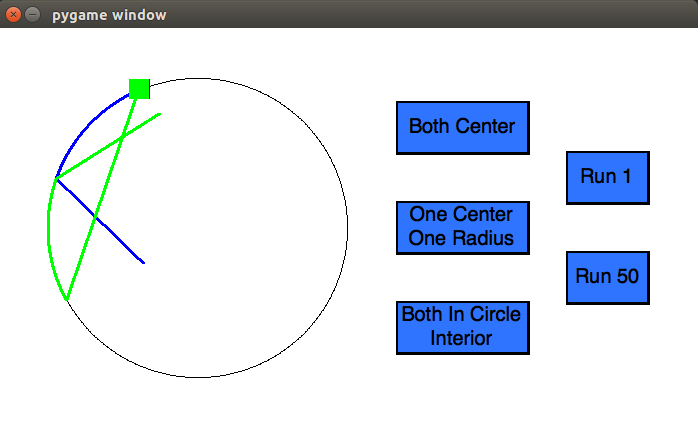
\includegraphics[scale=0.5]{images/scenario-3-4.png}}
        \end{center}
        
        
\end{document}